\section{Identification of code structure. Focus of analysis.}

Before proceeding into gathering the efficiency metrics, we need to study the application structure to decide the \textit{focus of analysis}.

The Focus of Analysis is the region of the application we select to study. We choose a region representative of the application, meaning that we usually discard initialization and finalization code. When the application presents repetitive patterns, such as an iterative pattern, we select a representative part instead of the whole region.

For doing so, we take a trace with one node and then with the useful duration view in Paraver, we try to identify patterns. Figure \ref{alyastructure} illustrates the useful duration view of Alya with one node. The x-axis represents time, the y-axis the processes, and the colour means the amount of time each process performs computation with a scale from green to blue, green means lower time and blue higher. We observe three phases, first an initialization phase, then an iterative pattern and finally a finalization phase. As the trace file generated is big and the iterations are constant, we decide to study just four iterations.

\begin{figure}[h]
  \centering
  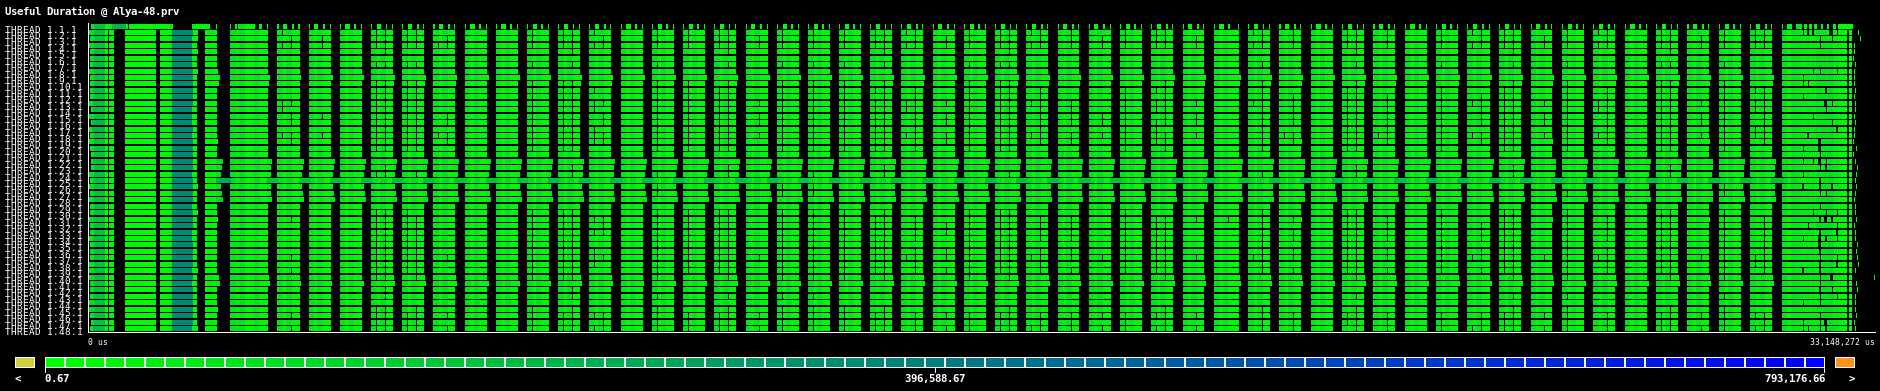
\includegraphics[width=1.0\textwidth]{structure-alya.w_legend}
  \caption[Alya structure]{Alya structure. Own compilation.}
  \label{alyastructure}
\end{figure}

Figure \ref{alyafoa} shows the \textit{focus of analysis}, as said, we focus on four iterations. We can see a notable difference of time in useful between processes, which suggests a load balance problem.

\begin{figure}[h]
  \centering
  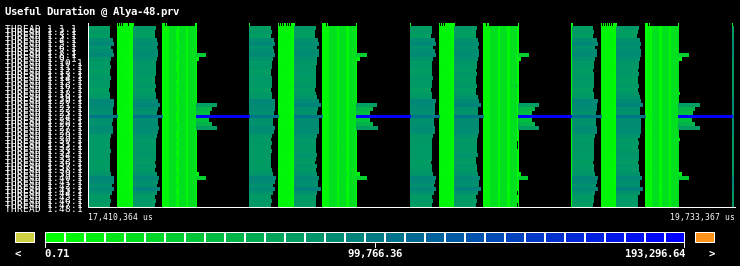
\includegraphics[width=1.0\textwidth]{foa-alya.w_legend}
  \caption[Alya focus of analysis]{Alya focus of analysis. Own compilation.}
  \label{alyafoa}
\end{figure}


